\begin{frame} 
\frametitle{Code: die Bausteine}

\only<2->{
\texttt{generate\_BBsignal}   
\only<3->{ : musste implementiert werden  } 

\smallbreak
\texttt{measure\_H} 
\only<4->{ : \texttt{getH.py} bereits gegeben in Python  }

\smallbreak
\texttt{compute\_Uquest}  
\only<5->{ : zum Teil gegeben in Matlab und Python  }

\smallbreak
\texttt{compute\_Uin} 
\only<6->{ : bereits gegeben in Matlab }

\smallbreak
\texttt{measure\_Uout} 
\only<7->{ : \texttt{writeAWG.py} und \texttt{readDSO.py} waren gegeben  }

\smallbreak
\texttt{compute\_a} 
\only<8->{ : bereits gegeben in Matlab }

\smallbreak
\texttt{compute\_K} 
\only<9->{ : bereits gegeben in Matlab und Python   }

\only<10->
{
	\begin{textblock}{20}(63,55)
    	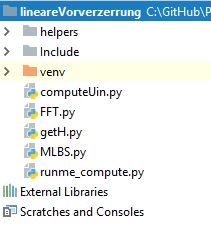
\includegraphics[scale=0.5 ]{slides/Gegeben/lineareFiles.JPG} 
	\end{textblock}	
	\begin{textblock}{20}(93,55)
    	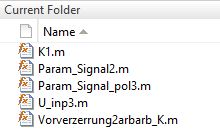
\includegraphics[scale=0.5 ]{slides/Gegeben/matlabFiles.JPG} 
	\end{textblock}	
}

}
\end{frame}
